% This is LLNCS.DEM the demonstration file of
% the LaTeX macro package from Springer-Verlag
% for Lecture Notes in Computer Science,
% version 2.2 for LaTeX2e
%
%\documentclass[12pt]{llncs}
%\documentclass[envcountsame,oribibl,11pt]{llncs}
\RequirePackage{amsmath}
\documentclass[runningheads,a4paper]{llncs}
%\documentclass[runningheads,a4paper]{llncs}
%\usepackage[hmargin=1in,vmargin=1.25in]{geometry} 

\usepackage{amsmath, amssymb}
\usepackage{algorithm,algorithmic}
\usepackage{makeidx}  % allows for indexgeneration
\usepackage{graphicx,epsfig,color}
\usepackage{boxedminipage}
\usepackage{multicol} 
\usepackage{enumerate}
\usepackage{diagbox}
\usepackage{float}
\usepackage[table]{xcolor}
\usepackage{multirow}
\usepackage{longtable}
%\usepackage{titlesec}

\setcounter{secnumdepth}{5}
% To use "Arial" font, use the following 2 lines
%\renewcommand{\rmdefault}{phv} % Arial
%\renewcommand{\sfdefault}{phv} % Arial

% The following statement specifies the amount of space between
% paragraphs. Other reasonable specifications are \bigskipamount and \medskipamount.
%\setlength{\parskip}{\smallskipamount}

% The following statement controls the line spacing.  
%\renewcommand{\baselinestretch}{1.0}

% TRACK CHANGE
% ------- Bar -------
%\begin{changebar}
% The proposed scheme
%\end{changebar}
% ------- Highlight -------
%\hl{scheme} 
% ------- Strikeout -------
%\st{framework}
%\usepackage{soul}
%\sethlcolor{green}
%\setstcolor{red}
%\usepackage[color]{changebar}
%\cbcolor{blue}

\begin{document}

%\bibliographystyle{abbrv}	% [1] A. Author. Article name, ...
\bibliographystyle{acm}	% [1] AUTHOR, A. Article name. ...
%\bibliographystyle{alpha}	% [Las98] Firstname Lastname. Article title. ... [alphabetical order]
%\bibliographystyle{apalike} 	% [Author, 1990]
%\bibliographystyle{amsplain}	% [1] Firstname Lastname, Italicized Article Name, ... 
								%        [authors in alpha order, underscore for repeated author]
%\bibliographystyle{ieeetr}	% [1] F. Writer. "Article name", ... [in order of reference]
%\bibliographystyle{plain}	% [1] Firstname Lastname. ...
%\bibliographystyle{siam}	% [1] A. AUTHOR, Italicized Article Name, ...
%\bibliographystyle{unsrt}	% [1] Firstname Lastname. Article name. ... [in order of reference]

%
\frontmatter          % for the preliminaries
%
\pagestyle{headings}  % switches on printing of running heads
\addtocmark{Title of The Paper} % additional mark in the TOC
%
\mainmatter              % start of the contributions
%
\title{A Survey on Trust in Autonomous Systems \\ 
}
%
\titlerunning{A survey on Trust}  % abbreviated title (for running head)
%                                     also used for the TOC unless
%                                     \toctitle is used
%
\author{\large Shervin Shahrdar and Mehrdad Nojoumian   %\inst{1} \thanks{Research supported by X.} 
%and Name-2 %\inst{2} \thanks{Research supported by X.}
}

\authorrunning{ Shervin Shahrdar  \& Mehrdad Nojoumian
}   % abbreviated author list (for running head)

\institute{
Department of Computer \& Electrical Engineering and Computer Science \\ Florida Atlantic University, Boca Raton, FL, USA \\
\email{sshahrda@fau.edu}, \url{www.shervinshahrdar.com} \\
\email{mnojoumian@fau.edu}, \url{http://faculty.eng.fau.edu/nojoumian/}
}

\maketitle
\begin{abstract}

\noindent As a result of the exponential growth in technology and computing in the past couple of decades, autonomous systems are becoming more relevant in our daily lives. As these autonomous systems evolve and become more complex, the concept of trust in such systems becomes a major challenge that affects the performance, and reliability of such systems. Many prior studies have indicated that currently, humans have a very low trust level in the fully autonomous robots. Similarly, the trust between autonomous systems plays a significant role in their performance. In this meta-analysis, we will explore various research and trust models to show why trust management is a very challenging aspect of future AI technologies.

\vspace{10pt}
\textbf{Keywords:} Trust Function, Reputation Systems, Autonomous Systems, Multi-Agent Systems
\end{abstract}

%\addtolength{\parskip}{1.6ex}
%\parindent 0pt

%-------
\section{Introduction} 
\label{ShervinTrustSurvey_introduction}
The rapid growth in technology has resulted in the automation of many day to day tasks that humans had to perform themselves just decades ago. From ATMs (Automated Telling machines) to industrial robots used in factories, automation continues to aid humans with repetitive, difficult, and monotonous tasks. This technological advancement introduces newer and more complex robotic concepts, and automated systems in different areas of our lives including our homes, daily commute, workspace, military, and many other areas every day.

As these automated systems evolve, their levels of complexity increase overtime, and their involvement in various aspects of human life introduces the concept of human-robot trust. Studies have indicated that one of the most important challenges for successful integration of advanced autonomous systems and AI technology in human civilization, will be the management and the development of this mutual trust \cite{beer2014toward}.

In this paper, we will provide a step by step, comprehensive analysis and explore various concepts and related studies, as well as experimental techniques proposed by researchers in this field, in order to understand how the human-robot trust management works, and how we can improve it. Additionally, we will explore the trust between autonomous systems (Agents) in section 3.

\section{Definitions}
\subsection{What is an Autonomous System?}
First, an autonomous system needs to be defined. This definition keeps changing everyday as the related technology grows exponentially \cite{schaefer2013perception}.

Merriam Webster dictionary defines `autonomy' as  ``The quality or state of being self-governing; especially: the right of self-government''. The concept of Autonomy has existed for thousands of years, in many different areas including philosophy, sociology, politics, and technology. In fact, the second part of the term Autonomous, \textsl{nomos}, means `law' in  Greek. An autonomous entity ``creates its own laws''. \cite{MerriamWebsterAtn}. 

We need to narrow down this definition, as this it is very broad and applies to many different areas and concepts. Perhaps the term that we are looking for is `autonomous robots'. Autonomous robots are defined as, ``intelligent machines capable of performing tasks in the world by themselves, without explicit human control.'' \cite{Bekey:2005:ARB:1088950}

\begin{figure}
	\centering
		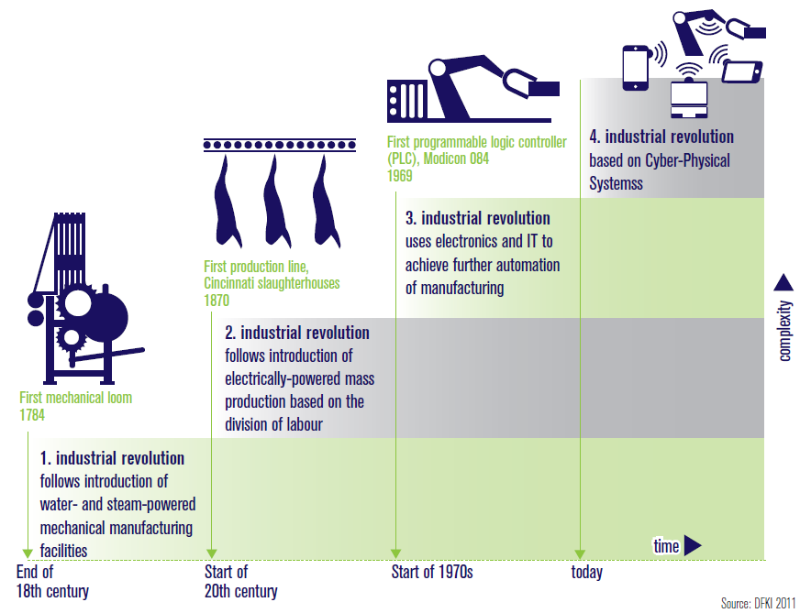
\includegraphics[width=\textwidth]{Figures/EvolutionOfAutomation.png}
	\caption{Evolution of Automation \cite{CyberSecurityInIndustry}}
	\label{Trust_Function}
\end{figure}
Although automation was introduced to human civilization many years ago, and widely used after industrial revolution in early 1800s \cite{IndustrialRevolution}, Autonomous systems, and Industrial Robots are relatively new terms that were introduced merely decades ago, and their definitions are evolving everyday, as technology advances. In this paper, our main focus will be on Autonomous Robots and Autonomous Agents which are a highly advanced form of automated machines that have a high degree of self-awareness, and are capable of independently performing tasks which were previously done by humans.

\subsection{What is Trust?}
`trust' is a concept that has many different definitions in various contexts such as psychology, sociology, and Economics. Currently, there is no uniform definition of `trust' in the context of psychology, or other areas \cite{adams2003trust}. Prior research indicates that there are over 300 definitions in various research areas, and in the context of Human-Robot relationships, which is our focus in this paper, there are more than 30 definitions. These definitions include `human interpersonal trust', `automation trust', `trust in software agents'', and many others \cite{schaefer2013perception}. 

Although there are complex definitions of trust documented based on the area of the research,  we shall focus on the simplest, domain-agnostic definition. A very simple, generic definition of `trust' would be: ``A firm belief in the reliability, truth, or ability of someone or something'' \cite{oxfordDicTrust}. If we consider this simple definition, then, in our research context, the definition of trust would be: ``A strong human belief in the reliability, truth, or ability of an autonomous system''. The `Autonomous system' in this case could be any kind of a self aware machine that has a high degree of autonomy. Some concrete examples would be human trust in self driving cars (SDC), autonomous planes, battlefield robots, rescue robots, autonomous software agents, and so on.

\section{Review of Literature: Trust in Autonomous Systems}
In this section, we will review, and categorize previous studies that are in the domain of human-robot trust relationship.

\subsection{Trust Between Humans and Autonomous Systems}

\subsubsection{Human-Robots}
As previously stated, many studies have shown that currently, the level of trust between humans and autonomous systems is very low. That means in serious situations, humans tend to not let fully autonomous systems take control. A study that explores the low level of human-robot trust, is done by Daniel Stormont (2008) \cite{stormont2008analyzing}. In this study, the factors that affect the trust between humans and robotic systems are analyzed. The study concluded that it is not just `trust' that determines the usability, but `confidence' also plays a significant role. One of the reasons the level of confidence in autonomous systems is very low is due to their low level of reliability. As cited in this paper, ``A 2004 study of commercially available ruggedized robots operating in
field conditions showed a mean-time-between-failures
(MTBF) of 12.26 hours and an availability rate of 37\%''\cite{carlson2004investigation}. This means, that if the robotic systems reduce their failure rate, their reliability will increase, thus, the human confidence and trust in them will increase. Of course this study was done in 2004. It is clear that due to recent advancements in robotic systems, the MTBF should be definitely less than 37\%. For example, when the first fatal car accident was reported for Tesla self driving cars, it became a topic of discussion in the media. Although these accidents are rare, companies like Tesla and Google learn the nature of the accident, and work on reducing the failure rate in the future models. \cite{TeslaFatalAccident}

In a study from 2004, Robin Murphy and his team introduced how rescue robots may be utilized, not only in combat but also in cases where victims are unable to be reached\cite{murphy2004robot}.  The success of these robots, however, depend on the trust of the victim in which they are assisting.  The purpose of a rescue robot is to localize the victim, check for vital signs, and to manage the victim until they are extricated.  The robots would be able to access victims in areas that have are defined as 'area denial situations,' or locations with greater depths or physical barriers that medical personnel could not reach without putting their lives in danger.  It is important that the victim allows the robot to help and collect data to provide an optimal recovery and assistance to the victim.  Analyzing this interaction allows for trust to be measured in life or death situations.

In his research, Mr.Stormont (2008) also believes that another factor affecting the trust between humans and fully autonomous systems would be their unpredictability. It is known that in various hazardous circumstances such as battlefields and rescue missions, the unpredictability of robots becomes a critical problem for human supervisors. It has been argued that the autonomous nature of robots, and their decisions making could be a positive trait, since they could react faster to certain dangers compared to humans, but the problem arises when life and death of humans will depend on the choices of a robot; Questions such as ``should life and death decisions be made
by an autonomous system?'' will emerge. In the 2008 study, a simulation of robots assisting firefighters in a hazardous fire situation was discussed. It was concluded that even though firefighters did not initially trust these helper robots, as the mission went on, and they got tired, their reliance and trust in the robots increased, as they helped them extinguish the fire. 
\begin{figure}
	\centering
		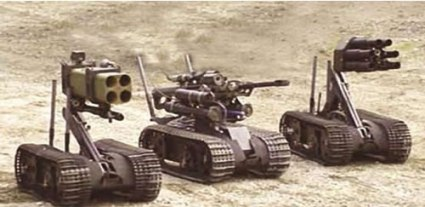
\includegraphics[scale=0.6]{Figures/3robots.jpg}
	\caption{Example of autonomous and semi-autonomous robots used in military \cite{autonomousArmedRobots}}
	\label{MilitaryRobots}
\end{figure}

Another study conducted by Mr. Babak Esfandiari and his colleague, Mr. Sanjay Chandrasekharan \cite{esfandiari2001agents} thoroughly examined and proposed ``simple
mechanisms for trust acquisition based on a very basic and general definition of trust.'' According this this study, the majority of views on the definition of trust are divided into two groups: Cognitive views, and mathematical views. Mr. Esfandiari argues that both of these views have something in common: both of them see `trust' as a variable, that also has a threshold for an action. This action is called cooperation. The mathematical definition of `trust' provided by this study is: ``Trust is a function T between any two agents of a set A of agents''. These agents can be humans, or robots, or autonomous systems, and so one. This study also provides a concept called `Trust Acquisition'. Given an example of previously defined mathematical function: T(Alice, Bob) (Trust between Alice and Bob), Trust Acquisition is described as ``the process or mechanism that allows the calculation and update of T. In our
definition, acquisition is not necessarily an 'increase' of T.''. This study provides various methods of Trust Acquisition:
\begin{enumerate}
	\item Trust Acquisition by Observation
	
	Mr. Esfandiari argues that Trust Acquisition can be obtained by performing `Bayesian Learning'. This means that agents observe, and consider that past actions of other agents, and decide whether to perform an action or not. This paper provides an example of two agents, RoboCop robots John and Mary. John has the ball, and is deciding whether or not pass the ball to Mary, or just shoot the ball himself. If John is able to review the past performances of Mary, and compares them with his own performance, and performs a statistical analysis, he will be able to make a decision.
	\item Trust Acquisition by Interaction
	
	In Trust Acquisition by Interactions protocol, agent 1 asks a bunch of pre-determined questions from agent 2. Agent 1 already knows the answer, thus, the trust will be acquired based on the the number of correct answers provided by agent 2.
	\item Trust Acquisition Using Institutions
	This study provides an example of humans trusting police officers wearing uniforms. If a person sees another person equipped with a gun who is wearing a uniform, he will automatically trust that person, because the trust is already established by the institution. However, if he sees a person not wearing a uniform and carrying a gun, he needs to make more calculations to trust this person.
	
\end{enumerate}


In a 2011 paper, Peter A. Hancock et al. provided a comprehensive analysis of factors affecting trust in ``Human-Robot Interaction (HRI)'' \cite{hancock2011meta}. This study categorizes factors that affect the trust in HRI into three different categories: human related, Robot related, and environmental variables, and each category has sub categories. Human related factors include training, expertise, situational awareness, demographics etc. Similarly, robot-related factors are behavior, dependability, reliability, level of automation, failure rates, false alarms, and transparency, and attribute based factors such as location, personality, adaptability, robot type, and Anthropomorphism (having human traits). Environmental factors include team work, culture, communication, shared mental models, task type, task complexity, multi-tasking, physical environment. This paper discovered that robot performance has the biggest impact on trust in the context of HRI, and tweaking the robot performance has a direct impact on trust. For example, if an autonomous robot improves its performance, the value of trust will increase.

\begin{figure}
	\centering
		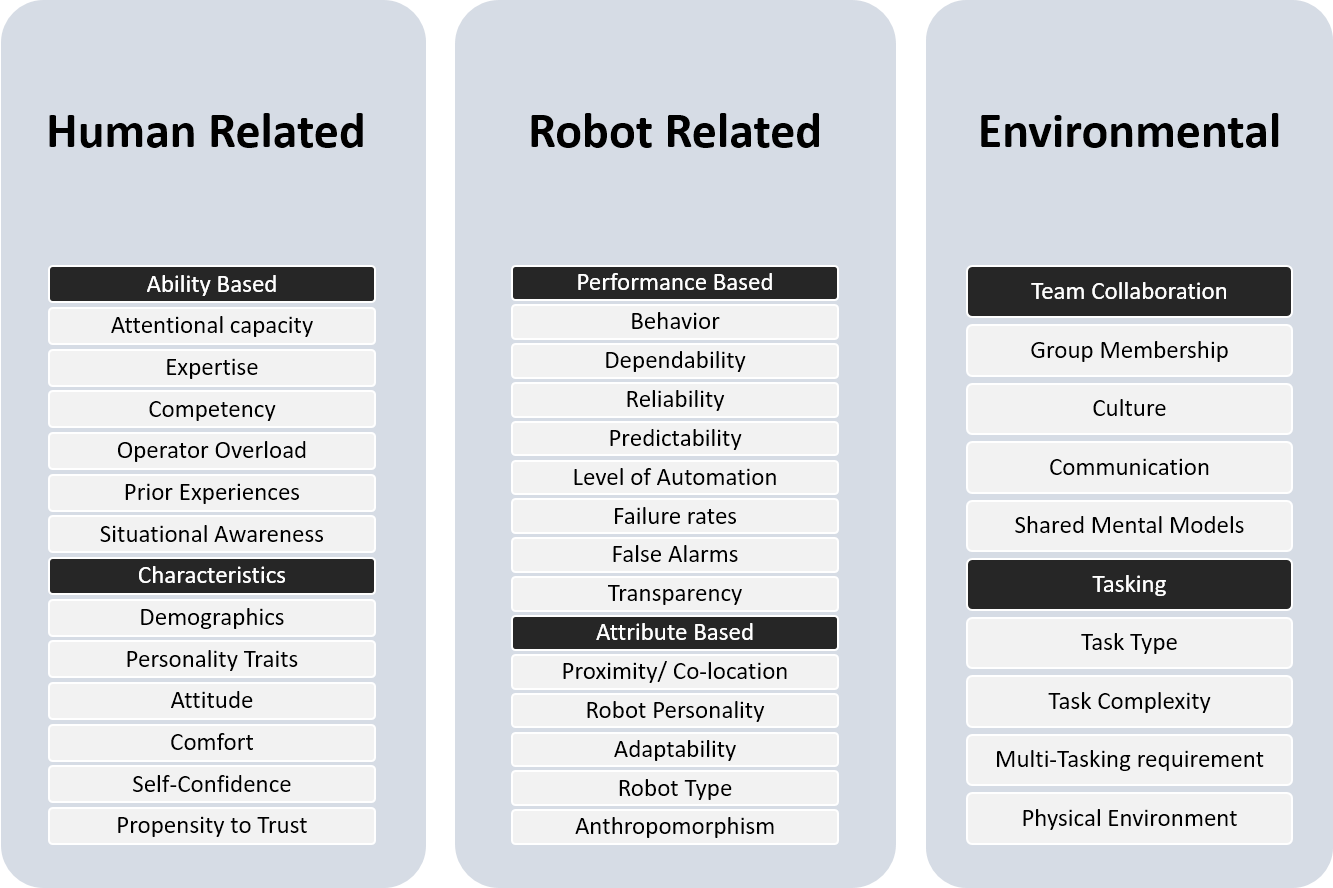
\includegraphics[width=\textwidth]{Figures/TrustFactors.png}
	\caption{Trust factors identified by Hancock \cite{hancock2011meta}}
\end{figure}

\newpage

Jacques Penders and his co-workers investigated HRI in `no-visibility' conditions \cite{penders2013enhancing}. No visibility condition in this context means that the human user might be visually impaired, or completely blind, therefore, they would have to completely trust the robot. This study also takes a look at the attributes in the design of robots that affect the ethical behavior of them. Additionally, this study analyzes the interaction of visually impaired person and their guide dog, and examines the variables that could be implemented in the design and behavior of robots to improve the human confidence in them. These variables include human dominance, cooperation overtime, and accountability.

In \cite{merritt2008not}, Stephanie Merritt at the University of Missouri examined the importance of taking differences in human behavior into consideration in the context of HRI. Ms. Merritt completed this empirical study by providing an experiment related to  X-ray screening. Subjects were asked to use a simulation software to detect dangerous items such as weapons, in different luggage. They given the options of scanning the x-ray image manually, and flagging it if they spot a suspicious item, or have a fictional autonomous system called  Automatic Weapons Detector(AWD) scan the image, and report any issues. This study concluded that the individual differences in subjects affects the value of trust in autonomous systems, even if the characteristics of the autonomous system is `constant'. Thus, this study suggests that future researchers in the field of HRI and trust should take human characteristics into consideration.

Raja Parasuraman and Christopher Miller investigated the concept of trust and etiquette in the domain of HRI \cite{parasuraman2004trust}. Given the fact that in many human-to-human social interaction scenarios, respect and etiquette highly influence the level of trust. Mr. Parasuraman and Mr. Miller argued that they also influence the perception of autonomous robots in humans. In this paper, etiquette is described as: ``the set of prescribed and proscribed behaviors
that permits meaning and intent to be ascribed to
actions.''. This study also provides an experiment related to the role of etiquette in HRI. In order to assess the influence of etiquette, test subjects used a flight simulator software called Multi-Attribute Task (MAT), and communicated with the autonomous system using different communication styles such as interrupting the user, being impatient, etc. The empirical evidence obtained by this experiment indicated that etiquette definitely influences the human trust, and reliability of autonomous robots.

A study done by Dingjun Li and his team in 2010 investigated how culture and appearance have an effect on trust\cite{li2010cross}.  The group sampled participants from who were from China, Germany, and Korea in order to properly analyze different cultural backgrounds.  The participants were asked to interact with the robot while it had customs from each of their countries.  The results were scaled based on likeability, engagement, trust, and satisfaction.  The outcomes demonstrated that the robot appealed differently to each of the participants, thus showing the need for increased concentration in different areas.  Producers may use this information to create their robots more unique to specific regions and cultures, thus improving trust and demand within the communities.

A research conducted by Ms. Rosemarie Yagoda and her research partner, Mr. Douglas Gillan, provided a mechanism for measuring the value of trust in the context of HRI \cite{yagoda2012you}. This measurement is based on multiple factors, including team configuration, team processes, context, task, and system. This trust scale measuring mechanism is based on two studies in this research. In this first study, subject matter experts, and previous studies were used to construct a `content validity assessment'. The second study examines the trust scales obtained from the first study. The results of these two studies were combined to create the `HRI Trust Measuring Tool'.


M. Itoh and partners conducted a study based on the effects of continuous and discrete malfunctions within autonomous systems in 1999\cite{itoh1999trust}.  The study was broken up into two parts.  The first section of the survey tested participants based on continuous and discrete faults separately, whereas the second part of the study intertwined the two malfunction types.  The experiments found a significant decrease in trust after five continous malfunctions.  However, there was no significant reduction in trust after one discrete malfunction.  The results of this study help companies see the path to how trust is dissipated, and how users will rely on autonomous systems based on the previous faults that occur.


In a 2014 paper, Yue Wang and partners investigated the human-robot trust in the context of underwater semi-autonomous robots \cite{wang2014human}. In order for the underwater robot to have a good performance, the person who is operating the robot needs to trust its autonomous capabilities. This study proposed a trust model that mainly deals with recording the robot's past performance, the human performance, and the fault rates of humans and robots. The semi-autonomous robot `YSI EcoMapper AUV' was investigated in this study specifically. Furthermore, MATLAB simulations indicate the effectiveness of this trust model.

In 1987, Bonnie Muir at the department of Psychology at University of Toronto, provided an analysis on the human-machine trust from a Psychological perspective \cite{muir1987trust}. This paper talks about ``Decision Support Systems'' (DSSs), and how trust is involved in the use of such systems. DSSs are computer programs that assist an individual, or an organization make decisions. These decisions include ranking important documents, buying and selling stocks quickly, choosing a target market, and many other important decisions \cite{decisionSupportTrust}. Since DSSs have a high impact on some critical decisions, the user's trust in such systems becomes a very important factor when designing  Decision Support Systems. Muir initially analyzed the Psychological trust models between humans, and used these models to provide a human-machine trust model. In this model, the concept of ``Trust calibration'' is introduced, in which, the user's have the responsibility of calibrating their trust based on the reliability of the DSS they are using. Muir suggests that when designing DSSs, there are certain factors and design goals that could contribute to better trust calibration. These factors are:
 \begin{enumerate}
 	\item \textbf{Aiming to improve the user's perception of trustworthiness of the DSS.}
 	This would require the user to completely understand how a DSS works, and become familiar with the predictability of the system's decisions. Muir suggest that this can be achieved by putting the user on a trial period of using a DSS, in order to improve the user's perception. A recommended technique is the use of a simulation environment so the user can freely explore the DSS without the fear of it making bad, or dangerous decisions.
 	\item \textbf{Modifying the DSS's ``Criterion of Trustworthiness''}
 In order to achieve this, the DSS has to provide a history of efficiency and good performance. It is recommended that users see statistical data such as ``System Performance''.
 	\item \textbf{Continuous identification and fixing the causes of poor trust calibration}
 In order to improve the trust between humans and the machines, the system (or developers) should be able to identify the root causes of bad trust calibrations, and fix them. This study indicates that some causes of low trust might be incorrect expectation of the users, therefore, the calibration training for the users is very important
 \end{enumerate}

A few years later, in 1994, Muir continued her research on human-machine trust by publishing a new paper with regards autonomous systems and human interventions when using them \cite{muir1994trust}. Muir claimed that nowadays, a lot of industrial and non-industrial systems are highly automated, and humans usually have a choice of letting the system do its job, or take manual control when they think they would have to. Muir claimed that the trust in the autonomous (or semi-autonomous) system might directly affect the number of times the users might intervene with the work of the autonomous system. In this study, Muir proposed a theoretical trust model that derives the role of trust between humans, and applies them to human-machine trust. The trust model provided by this paper includes the concept of ``Trust Calibration'', which is very similar to the concept presented in \cite{muir1987trust}. Muir, however, suggested that this trust model is purely theoretical, and needs experimental analysis to verify its effectiveness.

Muir continued her research on this topic, and published the second part of her previous publication (\cite{muir1994trust}) in 1996 \cite{muir1996trust}. In this study, two experiments were conducted, which were very similar to the experiment in \cite{lee1992trust}, simulations for a controlling milk pasteurization plant were created to test the major variables in human-machine trust, and to provide experimental analysis on the theoretical trust model proposed a few years earlier in \cite{muir1994trust}. The results of the experiments in this study indicated that the perception of ``Competence'' of an autonomous system correlates to the amount of trust a user can have in them. For example, if a user detected that the system might be incapable of doing its job (incompetence), they would manually take control of the system, thus, their trust would be drastically reduced. Another finding of this interesting study was that if the amount of the user trust in the system increases, the amount of monitoring the task reduces(Inverse relationship). This can be applied to trust in autonomous vehicles. If the driver has high amount of trust, their monitoring of the autonomous driving would reduce overtime, therefore, they would be able to do other activities such as reading or sleeping or watching TV while the autonomous system takes care of its job. Muir suggested that the findings in this research could be potentially used by the industry professionals to determine which properties of the autonomous system could have vulnerabilities that might display ``incompetence'', and lower user trust. By doing that, and predicting the patterns of user trust, they would be able to increase the overall effectiveness of the autonomous system.

In 1992, John Lee and Neville Moray explored the human-machine trust by studying the interactions of the users of a ``Semi-Automatic Pasteurization plant'' \cite{lee1992trust}. Based on the previous research, it had been known that the level of trust between humans and autonomous or semi-autonomous systems fluctuates depending on a variety of factors. For example, if was argued that some users didn't trust the new, semi-autonomous technology at all, and preferred to use the manual controls, instead of letting the autonomous system take care of the work. Some other users, interestingly, put ``too much'' trust in these systems, therefore, the risks of potential errors or faulty behavior caused by the system was possible. In the experiment provided by this paper, users were given the choices of operating a semi-automatic pasteurization plant for pasteurizing orange juice (simulation) using the manual mode, or the automatic-mode, or a combination of the mentioned two methods. This experiment indicated that the majority of users were able to adapt fairy quickly to this semi-automatic systems, however, when faulty behavior occurred, it was observed that the level of trust recovered more slowly. It was also concluded that the performance of the system significantly impacts the user's level of trust in the system.

Another compelling study that examines the role of trust in Decision Support Systems (DSSs) and autonomous aids is done by P.Madhaven and his colleague, D.A Wiegmann in 2007 \cite{madhavan2007similarities}. Since the role of DSSs, especially autonomous aids for humans for making critical decisions has been significantly increasing over time, this paper introduced a complex framework which sheds some light on the process that needs to take place for the users' trust in autonomous aids increase over time. This trust framework utilizes the psychological attributes that affect the trust between humans and uses them to provide a set of instructions for the DSS so that the human trust in DSSs would increase. This research's outcome contributed to the identification of several important psychological factors such as favoritism (human partners vs. robot partners), and subjective bias in users, which influence human-robot trust relationship, and thus, critical to the development of valuable DSSs, and other autonomous systems require the users' trust.

In a 2011 study, Mahtab Ghazizadeh and her colleagues worked on shedding some light on the users' acceptance of automated systems and proposed a model called ``Automation Acceptance Model'' (AAM) \cite{ghazizadeh2012extending}. This model employs concepts from research done in the Cognitive Engineering (CE), and Information system (IS) domains. In CE, most of the research focus has been on the ``Compatibility'' of new technology with everyday human use, and in IS, the focus has been on the user acceptance of new technologies. Therefore, Ghazizadeh morphed the concepts from these two domains and constructed AAM to use them in the context of automation, and assess the effects of user attitude and behavior on the amount of trust in automation. Although very complex, AAM is claimed to be very flexible and can be adapted to various automation types (e.g SDCs, autopilots etc.).

Collaboration between autonomous robots and humans in military operations has been growing significantly in the past few years (e.g. military drones, bomb defusing robots,  etc.). Therefore, trust is a major factor impacting the collaboration between humans and robots. In a 2007 paper, Amos Freedy and colleagues worked on creating a model called ``Collaborative Performance Model'' \cite{freedy2007measurement}. This model aims to capture the essential components of the collaboration between robots and humans. This performance model uses the following concepts from other research areas and combines them to enhance this model:
\begin{enumerate}
	\item Psychology of Team Performance
	\item Unmanned Autonomous Systems
	\item Mixed-Initiative Systems
	\item War-fighting behavior
\end{enumerate}

To test this trust model, Freedy conducted a simulated experiment in an environment called Mixed Initiative Team Performance Assessment System (MITPAS). This simulation environment enables the researchers to study the behavior and performance of humans and robots in combat zones. This experiment concluded that as the level of competence of robots decrease, their trustworthiness also decreases, and humans start controlling them using the manual overrides more often. Additionally, if the robots are less competent, the overall mission time would also increase. Overall, this study concluded that measuring the trust in the context of human-robot collaboration can be very beneficial, and the use of simulation environments such as MITPAS can help researchers understand human-robot collaboration better.

In a 1996 paper, I. Dassonville and colleagues investigated the issue of trust within the context of a ``Teleoperation System'', and attempted to analyze the role of trust in relationships of humans, and extended this trust to the human-machine system \cite{dassonville1996trust}. This study also conducted experiments on the role of self-confidence in the human-machine relationship. A teleoperation system is a type of system in which the human operators can operate a machine or a system from a distance. This study describes such system and argues that it is simply composed of three components:
\begin{enumerate}
	\item \textbf{Master Universe}
	The master universe is essentially the environment in which the operator resides in. An example of this would be a military drone operator sitting in a container in the middle of a desert, controlling a strike drone somewhere far away in a combat zone. 
\item \textbf{Slave Universe}
Similarly, the slave universe is the environment in which the machinery or the system resides, that is to be operator by the operator. This universe is made of hardware and a bunch of sensors.
\item \textbf{Space between Master Universe and Slave Universe}
This space between the Master Universe and the Slave Universe contains data transmission (e.g. Internet), fast computers, and Decision Control Systems (DCSs).
\end{enumerate}

For the experiment in this paper, a simulated experiment was conducted using an operator using a joystick (Master Universe) connected to a computer (Space in Between) to control a cursor on the screen (Slave Universe). Operators were later given a questionnaire regarding their experience with the simulator. This experiment was conducted on two student populations of literature studies, and scientific studies. The experiment concluded that the first population appears to be more self-confident in operating the machine than the second one, however, the levels of trust in the system appears to be the same.

\subsubsection{Human-Self Driving Cars (SDCs)}
Autonomous driving has been advancing exponentially in the recent years due to technological advancements in AI, mechanics and advanced sensor systems. Car manufacturers such as Google, Tesla, Mercedes-Benz, Ford, and many others have already created commercially available semi-autonomous cars, and fully autonomous prototypes, and they expect mass production of self driving cars (SDCs) in the early 2020s \cite{driverlessFutureForcast}. One major challenge in popularizing SDS in the US and the world would be the high level of distrust of average consumers in fully automated vehicles.

Daniel Howard at UC Berkeley (2013) \cite{howard2014public} explores the factors affecting the trust between humans and SDCs, and attempts to examine the attitude of average consumers towards SDCs in Berkeley, California. Mr. Howard's research indicates that most consumers have positive feelings toward the ease of use that comes with SDCs. In a fully autonomous vehicle, they wouldn't have to feel frustrated when driving in heavy traffic, or finding parking in a busy area due to the benefit of multitasking. One can imagine that at some time in the near future, commuters will be able to take naps, or watch movies while the SDC drives them to wherever they desire. Mr. Howard's also discovered that most individuals have concerns regarding the cost, liability, and the potential loss of control of SDCs. This study also indicated that factors such as level of income and gender affect the consumer's concerns. For example, subjects with higher levels of income were more concerned about liability as opposed to subjects with lower levels of income that were more concerned about the control of SDCs.

An experiment  conducted by William Payre and his team analyzed how alternating levels of trust would impact a driver's reaction time \cite{payre2016fully}.  The purpose of this experiment was to test the time between Manual Control Recovery (MCR) when emergency situations arose with Fully Automated Driving cars (FAD's).  Cars that are FAD's are certified and eligible to be used by drivers with a standard driver's license.  Nonetheless, the drivers are still accountable for their vehicle and regaining MCR in case of emergency, as well as being in the drivers seat with their seat belt buckled at all times.  Participants were asked to take a questionnaire prior to the simulation, as well as another one after the simulation.  The simulation was divided into three rounds that allowed researchers to test the reaction time between users being warned 30 seconds ahead of time to engage in MCR, and drivers upon emergency situations, in which they would have no warning ahead of time.  The first round allowed users to familiarize themselves with the controllers, the second had users starting the cars, as well as getting them up to 130 kmp until they were signaled to commence the FAD system and then engage in MCR, and the third gave users an emergency situation in which drivers had to engage in MCR as quickly as possible.  This study demonstrated that higher trust levels in the FAD's resulted in slower reaction times, which can create a hazardous environment for drivers who are complacent.  This experiment helped companies become more aware of the problems that over trust can cause, as well as simulate ideas for courses regarding gaining knowledge in MCR.

Michelle Carlson and her team, in a 2014 paper, provided a statistical analysis in the domain of autonomous vehicles and autonomous diagnostic systems \cite{carlson2014identifying}. Their goal was to identify the major factors that impact level of trust in self driving cars and autonomous medical systems. In this study an online survey was performed in which subjects were asked about various scenarios related to self driving cars. They were also asked about the use of IBM Watson in critical medical situations (e.g determining types of cancer). It was discovered that most test subjects were having concerns regarding the past performance of the car, reliability, errors, software/hardware failure, and the liability manufacturer of the car (e.g Google, or a lesser-known company). Similarly, it was discovered that the top factors that affect the trust in the use of IBM Watson in critical medical situations are the accuracy and past performance among many other factors. This indicates that regardless of the domain, most people tend to prioritize safety, accuracy, and failure rate when trusting an autonomous system.

In a similar study \cite{kyriakidis2015public}, Miltos Kyriakidis and his team created an international questionnaire related to the public opinion of automated driving. Questions included concerns, acceptance, and willingness to buy the car. Among the 5000 responders from 109 countries, most subjects agreed that fully automated self driving cars have the potential to be very popular among consumers by 2050. It was discovered that most subjects were concerned about safety, malicious activities/hacking, and legal issues related to autonomous driving. Mr. Kyriakidis also discovered that most of the subjects that were more educated, had more income, and were located in developed countries, were mostly uncomfortable about the self driving car transmitting data to external sources, and were concerned about the misuse of the transmitted data.

A 2015 study by Michael Wagner and Philip Koopman explored the possibilities of developing trust in Self Driving Cars using tools and techniques that are currently available \cite{wagner2015philosophy}. This study argues that fully autonomous Driving Cars aim to make our lives easier, and reduce the number of accidents. However, in many situations such as unpredictable hazards, and intense weather situations, the human driver's reactions are superior. This is one of the major factors that affects the human trust in Self Driving Cars. It is stated that testing is a critical aspect of determining if the car is trustworthy enough to be on the road, or has the potential to develop its trust over time. This paper also claims that these cars use Machine Learning and Image Processing to provide some functions, like detecting pedestrians. It was argued, however, that Self Driving Cars need a very high accuracy in their algorithms (close to 100\%), but Machine Learning algorithms are not capable of producing such accurate results. Mr. Wagner and Mr. Koopman bring to light a new software testing philosophy based on philosopher, Karl Popper's concept of `Falsification'. Falsification means: ``For any hypothesis to have credence, it must be inherently disprovable before it can become accepted as a scientific hypothesis or theory.''\cite{falsifiability}. Falsifiability helps testing because it causes testers to discover more flaws and vulnerabilities in Self Driving Cars. Thus, by improving, and reliability, the trust in them will increase over time.

In 2004, Ananth Uggirala and her team began a study that would analyze trust with the user being given information about the capacity of the autonomous vehicle\cite{uggirala2004measurement}.  This study aimed to decrease uncertainty in order to optimize system performance by having the user be knowledgeable of the functions the system is able to executed.   The participants went through a training to gain familiarity with the system and afterward were asked to analyze the reference lines.  The reference lines were of varying lengths and participants had to judge whether or not the vehicle would be capable of efficiently completing the given functions given the reference lines.  The study concluded that when users are given knowledge then competence and trust increases.


Tove Helldin and colleagues at the University of Skövde in Sweden conducted a study related to the ability of SDCs in snow conditions \cite{helldin2013presenting}. In this study, 59 drivers were chosen to sit in an autonomous simulator cockpit. One group of drivers were given information about the risks and uncertainties of the SDCs when driving in heavy snow conditions, and the other group of drivers, were not given any information regarding the ability of the SDC. This experiment indicated that the group of drivers that were provided with the information about the risks and uncertainties did not trust the SDC, and preferred to override the system to manually drive the car. The other group, however, were not as prepared to override the autonomous system to drive the car manually, and had more trust in the system.

In a study, Monika Hengstler and colleagues investigated the trust in AI applications, primarily focusing on autonomous vehicles and medical assistance devices (MAD) \cite{hengstler2016applied}. In this paper, Ms. Hengstler argued that currently, there is a large amount of human skepticism and distrust in fully AI applications. Although it has been known that in the world of AI, we have strong AI, and weak AI, the current industries have been using weak AI to implement commercial applications and products for the consumers to use. The main reason for this is because strong AI is still at its early phases of development (It is still very far from something like the Terminator's Skynet). Considering the role of trust between humans, and how it is similar to human-machine trust, this study identified that the two major industrial areas directly affected by society's distrust in AI and autonomous systems are autonomous vehicles such as SDCs, autonomous trains, transportation services, and medical assistant systems such as IBM's Watson - An AI software capable of understanding natural language and solving problems - and other applications in the domain of healthcare, and proceeded to provide case studies and case by case analysis by interviewing industry's professionals and subject matter experts. It was concluded that in the case of autonomous vehicles, vehicle safety, on top of everything, affects the human level of trust in them. The second major factor, was found to be ``Data Security''. Data security in this case means how secure, and correct the information perceived by the sensors and how secure is the data processed by their system. In medical autonomous systems, it was concluded that the top concern among consumer is privacy. These medical assistant applications might contain sensitive information stored in their databases regarding patients and care about their privacy. Therefore, this study suggests that in order to improve the trust between humans and autonomous systems, future research, and focus of the industry should shift towards the above issues.

In a similar paper, Ann-Marie Nienaber and her partner, Gerhard Schewe conducted a research on the significance of perceived risk reduction in new, innovative products vs enhancing trust in the new product \cite{nienaber2014enhancing}. After collecting data from 490 subjects and analyzing their responses, it was concluded that working on improving the trust in the new product is more important than just focusing on risk reduction. This claim was supported by the fact that the test results trust in new products by consumers appears to be more subjective, and ``decisive'', therefore, it is recommended for the companies creating new, innovative products to not just reduce the perceived risks that comes with the product, but to work with potential customers, and help them increase their trust. For example, in the case of SDCs, this concept can be applied. Car manufacturers working on creating fully autonomous vehicles not only should work on reducing the perceived risks of driving a SDC, but they should also work on increasing their customers' trust in SDCs. Perhaps this can be achieved by setting up many demos of SDCs for general public, or even simulations for users who are afraid of even trying SDCs. This will improve the overall trust in the product, and thus, guaranteed increase of sales. Another interesting finding by this study was that the general dislike of new, unknown, and innovative products has ``no influence on the
relationship between contact intensity and relationship commitment''. This is a very unique, and interesting conclusion, because the majority of papers in the domain of human-machine trust claim the opposite.

Many papers in the domain of trust and HRI suggest that the users' subjective view of new technologies and their level of acceptance of them plays a significant role in the usage and popularity of such technologies. E-Commerce is one of the examples of fast growing technologies that used to be less popular (back in the 1990's) perhaps due to lack of trust in them, or fear of fraud. Nowadays, E-Commerce giants such as eBay and Amazon are widely used and accepted among consumers around the world. In a study, Paul Pavlou investigated the consumer acceptance and trust in E-Commerce and proposed a theoretical model that aims to reduce the user's uncertainty of buying and selling products online by integrating trust and ``perceived risk'' \cite{pavlou2003consumer}. To develop this model, Pavlou utilized two important concepts of Theory of Reasoned Action (TRA) and Technology Acceptance Model (TAM) to mathematically measure the user's acceptance and their online behaviour when interacting with Business to Consumer  (B2C) E-Commerces. In the described model, several factors affect the amount of users' trust in the E-Commerce platform they want to use to sell or buy products. These factors include ``Percieved Ease of Use'', ``Percieved Usefulness'', and ``Percieved Risk". If a user has the correct amount of the described elements, their trust in the product will increase. Thus, they will be more likely to conduct a transaction. Although this model is aimed to improve the users' trust in E-Commerce, we argue that the concepts discussed in this paper are very similar to the studies conducted on trust and HRI. For instance, if a consumer is reflecting on whether they should purchase a new autonomous vehicle or not, they would assess the vehicle's ease of use -how easy it is to just not drive during crazy rush hours- and its usefulness, and the risks associated with driving autonomous vehicles.

\begin{figure}
	\centering
		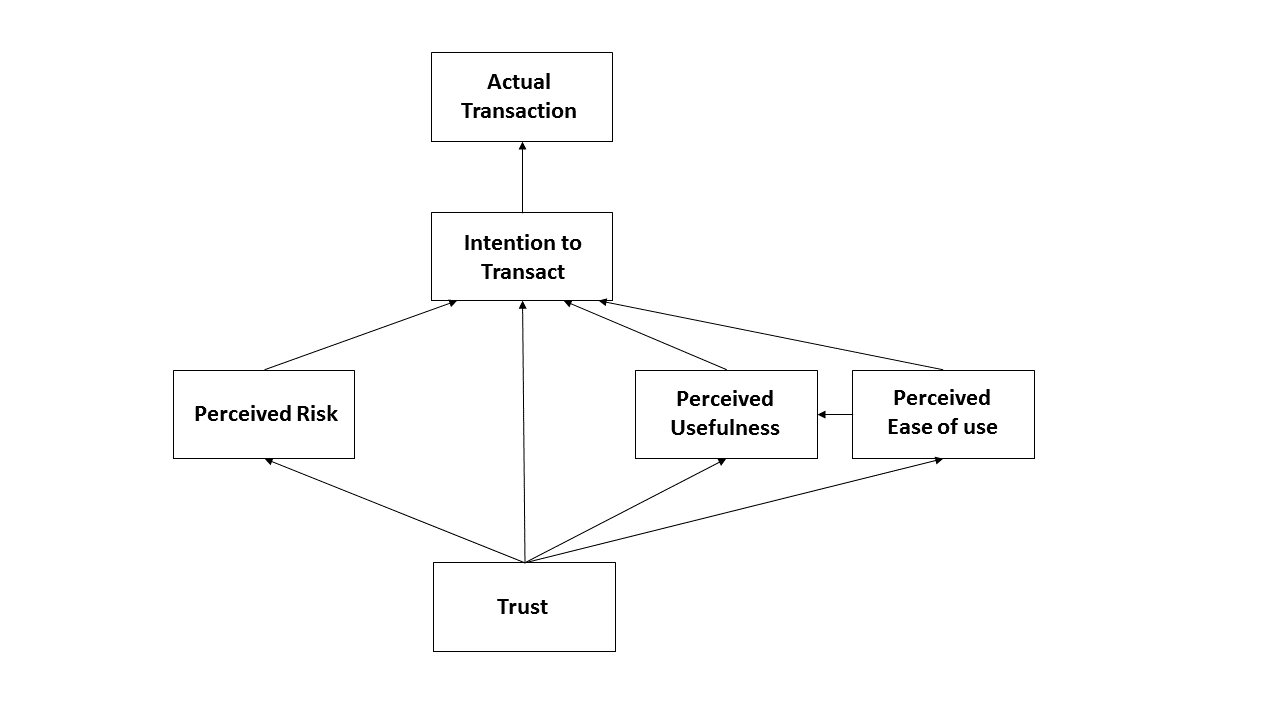
\includegraphics[width=\textwidth]{Figures/ECommerceTrust.png}
	\caption{Trust model described in \cite{pavlou2003consumer}}
\end{figure}

\subsubsection{Human-Autopilot Modes}
Scott Winter and colleagues \cite{winter2015indian} explored this low level of trust in the context of humans trusting autonomous aircraft. Subjects were asked if they preferred to be on a commercial plane with two pilots (a pilot and a copilot), a plane with a pilot in the cockpit and the copilot remotely working, or a plane with both pilots remotely controlling the aircraft. Mr. Winter and colleagues discovered that the subjects express a high degree of discomfort if they were on a fully autonomous commercial plane with both pilots just overseeing the movements and controlling the airplane remotely. They also discovered that subjects also expressed a low level of trust when only one pilot is in the cockpit and another one controlling the aircraft remotely. In this study, it was also concluded that the level of trust between humans and autonomous aircrafts is potentially related to the culture of humans. For example, it was discovered that test subjects from India feel more comfortable if they were on a fully autonomous aircraft, as opposed to subjects from the United States. Mr. Winter and colleagues found out that this difference could be due to the collectivist Indian culture, as apposed to the Individualist American culture.

Vadim Butakov and his colleague, Petros Ioannou, in \cite{butakov2015driving} suggest that the level of comfort and trust of users will increase if the design and dynamics of autopilot systems in cars are closer to what they are used to in regular cars. In this study, Mr. Butakov and Mr. Ioannou analyze and present a methodology that allows custom modification of autopilot modes such as  Adaptive Cruise Control (ACC) and automatic lane change systems based on individual preferences. They also support their proposed methodology by collecting data from an experimental vehicle.

At the The European Organization for the Safety of Air Navigation (\cite{kelly2003guidelines}), a study was conducted on the human trust in air trafic management systems (ATMs), and provides guidelines and strategies to improve this trust over time. This paper argues that currently, air traffic control operators use many automated and semi-automated computer tools, and it is expected that the use of automation in this context will rise in the near future. Thus, operators will have to trust highly autonomous (or fully autonomous) ATMs such as radar systems and communication tools. The procedure to improve the mentioned trust is broken down in multiple ``development phases'':
\begin{itemize}
	\item Developing ATMS using experienced air traffic controllers
	\item Providing high quality simulations
	\item Providing training for the controllers
	\item Transitioning period for the controllers
	\item Keeping the old technology in case failure
\end{itemize}


\section{Summary}

%\begin{table}[]
%\centering
%\caption{My caption}
%\label{my-label}
\begin{center}
\setlength\LTleft{0pt}
\setlength\LTright{0pt}
%\begin{longtable}{@{\extracolsep{\fill}}|c|c|l|c|c}
\begin{longtable}{|c|c|p{4cm}|p{2cm}|p{2cm}|}
\hline
\multicolumn{5}{|c|}{List of Studies}                                                                                               \\ \hline
Category                        & Study & \multicolumn{1}{c|}{Summary}    & \multicolumn{1}{c|}{Technology} & \multicolumn{1}{c|}{Focus} \\ \hline
\multirow{8}{*}{Human - Robots} 
	& \cite{stormont2008analyzing}    
	&  Confidence plays an important role as well as trust,\ and The unpredictability of the robot affects trust  
	& Computer simulation based on a firefighting scenario                        
	& Military, Hazardous environments
	\\ \cline{2-5} 
	& \cite{esfandiari2001agents}     
	& Mathematical definition for trust, where trust is a variable T. Trust acquisition is the process or mechanism that allows the calculation and update of 'T'
	& trust propagation model                      
	& Math-based trust propagation. Trust acquisition
	\\ \cline{2-5} 
	& \cite{hancock2011meta}
	& The performance of the robot has the biggest impact on trust in the context of HRI
	& N/A (meta-analysis)
	& HRI
	\\ \cline{2-5}
	&  \cite{penders2013enhancing}
	& In order to enhance trust in HRI, a number of design choices need to be made
	& visually impaired person and a guide dog
	& Improving trust in HRI
	\\ \cline{2-5} 
	& \cite{merritt2008not}
	& Different people have different levels of trust toward robot despite its constancy
	& X-ray screening simulation             
	& User perceptions of trust
	\\ \cline{2-5} 
	& \cite{parasuraman2004trust}
	& Etiquette affects human trust and the reliability of autonomous robots
	& Flight simulator
	& Impact of etiquette on trust
	\\ \cline{2-5} 
	& \cite{yagoda2012you}
	& Created the HRI `Trust Measuring Tool'
	& Subject Matter Experts (SMEs)                
	& Trust measurement
	\\ \cline{2-5} 
	& \cite{wang2014human}
	& If the human trusts the robot, its performance increases
	& YSI EcoMapper autonomous underwater robot         
	& Semi-autonomous mutual trust
	\\ \hline
\multirow{5}{*}{Human SDC}      
	& \cite{howard2014public}  
	& Most consumers like SDC's. Different people have different trust issues                     
	& Survey based on a 10 minute video                        
	& Perception of user's trust in SDCs
	\\ \cline{2-5} 
	& \cite{carlson2014identifying}
	& Most people tend to prioritize safety, accuracy, and failure rates when trusting an autonomous system                       
	& Surveys using  Survey Monkey and Amazon’s Mechanical Turk                  
	& Trust in Automated Cars and Medical Diagnosis Systems               
	\\ \cline{2-5} 
	& \cite{kyriakidis2015public}
	& The geographic positioning and education of consumers affects the premises of their trust 
	& Internet-based survey                    
	& User willingness to buy SDCs
	\\ \cline{2-5} 
	& \cite{wagner2015philosophy}    
	& Users testing; relying and improving will increase their trust in the robot 
	& N/A (survey of existing methods)         
	& Safety for SDC software based on 'falsificationism'
	\\ \cline{2-5} 
	& \cite{helldin2013presenting}
	& If people know about the problems of a robot, they will probably override it to avoid them            
	& Driving Simulator by Volvo  
	& The uncertainty of SDCs in various scenarios            
	\\ \hline
	
	\multirow{2}{*}{Human-Autopilot Modes}    
	& \cite{winter2015indian}
	& Culture affects trust                        
	& Internet based survey               
	& Trust in autonomous and semi-autonomous auto pilot systems        
	\\ \cline{2-5} 
	& \cite{butakov2015driving}
	& People have an easier time trusting familiar things.                   
	& Data collection from an experimental SDC
	& Autopilot personalization
	\\ \hline
	
e

%\end{tabular}
\end{longtable}
\end{center}

\section{Open Problems, Future Directions and Concluding remarks}
%\bibliographystyle{abbrv}
\bibliography{ShervinTrustSurvey}

\end{document}

